\documentclass{article} % kind of document 
\usepackage[utf8]{inputenc} %encoding of choice
\usepackage[american]{babel} %language of choice
\usepackage[p,osf]{cochineal}
\usepackage{fancyhdr} %for header
\usepackage{amsmath, tabu} %math mode
\usepackage{mathtools}
\usepackage{extarrows} % for more options with arrows
\usepackage{amssymb} %math symbols
\usepackage{dsfont} %specifically for the indicator function symbol
\usepackage{xcolor} %to color text
\usepackage{amsthm} %math theorem
\usepackage{tikz}
\usepackage{caption}
\usepackage{multirow}
\usepackage[bottom]{footmisc}
% \usepackage[dvipsnames]{xcolor}
\usepackage{enumerate} %make lists
\usepackage{graphicx} %insert images
\usepackage{float} %to fix image position
\usepackage{moreverb} %to make boxes
\usepackage{hyperref} %to create hyperlinks
\usepackage{lipsum} %lorem ipsum package
\usepackage{setspace} % to use singlespace below in the solution environment
\usepackage[shortlabels]{enumitem}
\usepackage{parskip}
\usepackage[us]{datetime} %package for setting due date in US format
\newdate{duedate}{20}{10}{2021} %to set a due date
\allowdisplaybreaks
\usepackage[margin=1in]{geometry}
\pagestyle{fancy}
\usepackage{jlcode}

\lhead{Due: \displaydate{duedate}}
\chead{ECON 899 -- Problem Set 6}
\rhead{Danny, Hiroaki, Mitch, Ryan, Yobin}


\DeclareMathOperator*{\E}{\mathbb{E}} %ease of writing e and E
\newcommand{\e}{\mathrm{e}}
\newcommand{\ct}{\mathsf{c}}
\newcommand{\Z}{\mathbb{Z}}
\newcommand{\R}{\mathbb{R}}
\newcommand{\N}{\mathbb{N}}
\newcommand{\ifn}{\mathds{1}}
\newcommand{\X}{\mathbf{X}}
\newcommand{\Y}{\mathbf{Y}}
\newcommand{\one}{\mathbf{1}}
\newcommand\numberthis{\addtocounter{equation}{1}\tag{\theequation}}
\newcommand*\widebar[1]{\overline{#1}} % to get a widebar
\theoremstyle{definition}
\newtheorem{theorem}{theorem} % Theorem display format
\newtheorem{problem}[theorem]{Exercise} % Problem display format, last bracket sets display choice

\newenvironment{solution}[1][Answer]{\begin{singlespace}\underline{\textbf{#1:}}\quad }{\ \rule{0.3em}{0.3em}\end{singlespace}} % Answer format

\newenvironment{solutions}[1][Proof]{\begin{singlespace}\underline{\textbf{#1:}}\quad }{\ \rule{0.3em}{0.3em}\end{singlespace}} % Answer format

\begin{document}
Tasks:
\subsubsection*{Task 1}
Solve both versions of the model presented above. Use the parameter values in the calibration section of section 1 for both versions.
\begin{solution}
Our code is attached in the appendix.
\end{solution}
\subsubsection*{Task 2}
Compute the following model moments and fill in the table. Are they any different across model specifications? If yes, try to explain intuitively what drives the differences.
\begin{solution}
	The table is the following. 
	\begin{center}
	\begin{tabular}{ccccc}
	variable & Standard & TV1 Shock $\alpha$ = 2.0 & TV1 Shock $\alpha$ = 3.0 & TV1 Shock $\alpha$ = 1.0\\
	Price Level & 0.739 & 0.725 & 0.728 & 0.713\\
	Mass of Incumbents & 8.321 & 8.829 & 8.207 & 10.336\\
	Mass of Entrants & 2.639 & 3.033 & 3.218 & 2.756\\
	Mass of Exits & 1.662 & 2.132 & 2.09 & 2.132\\
	Aggregate Labor & 179.834 & 183.024 & 181.198 & 187.775\\
	Labor of Incumbents & 142.627 & 142.497 & 137.744 & 152.541\\
	Labor of Entrants & 37.207 & 40.527 & 43.455 & 35.234\\
	Fraction of Labor Entrants & 0.207 & 0.221 & 0.24 & 0.188\\
	\end{tabular}
	\end{center}
\end{solution}

\subsubsection*{Task 3}
Plot the decision rules of exit in all model specifications you have solved. Are they any different? If yes, try to explain intuitively what drives the differences.
\begin{solution}
Figure \ref{T3} displays the results.
	\begin{figure}[htbp]
	\begin{center}
	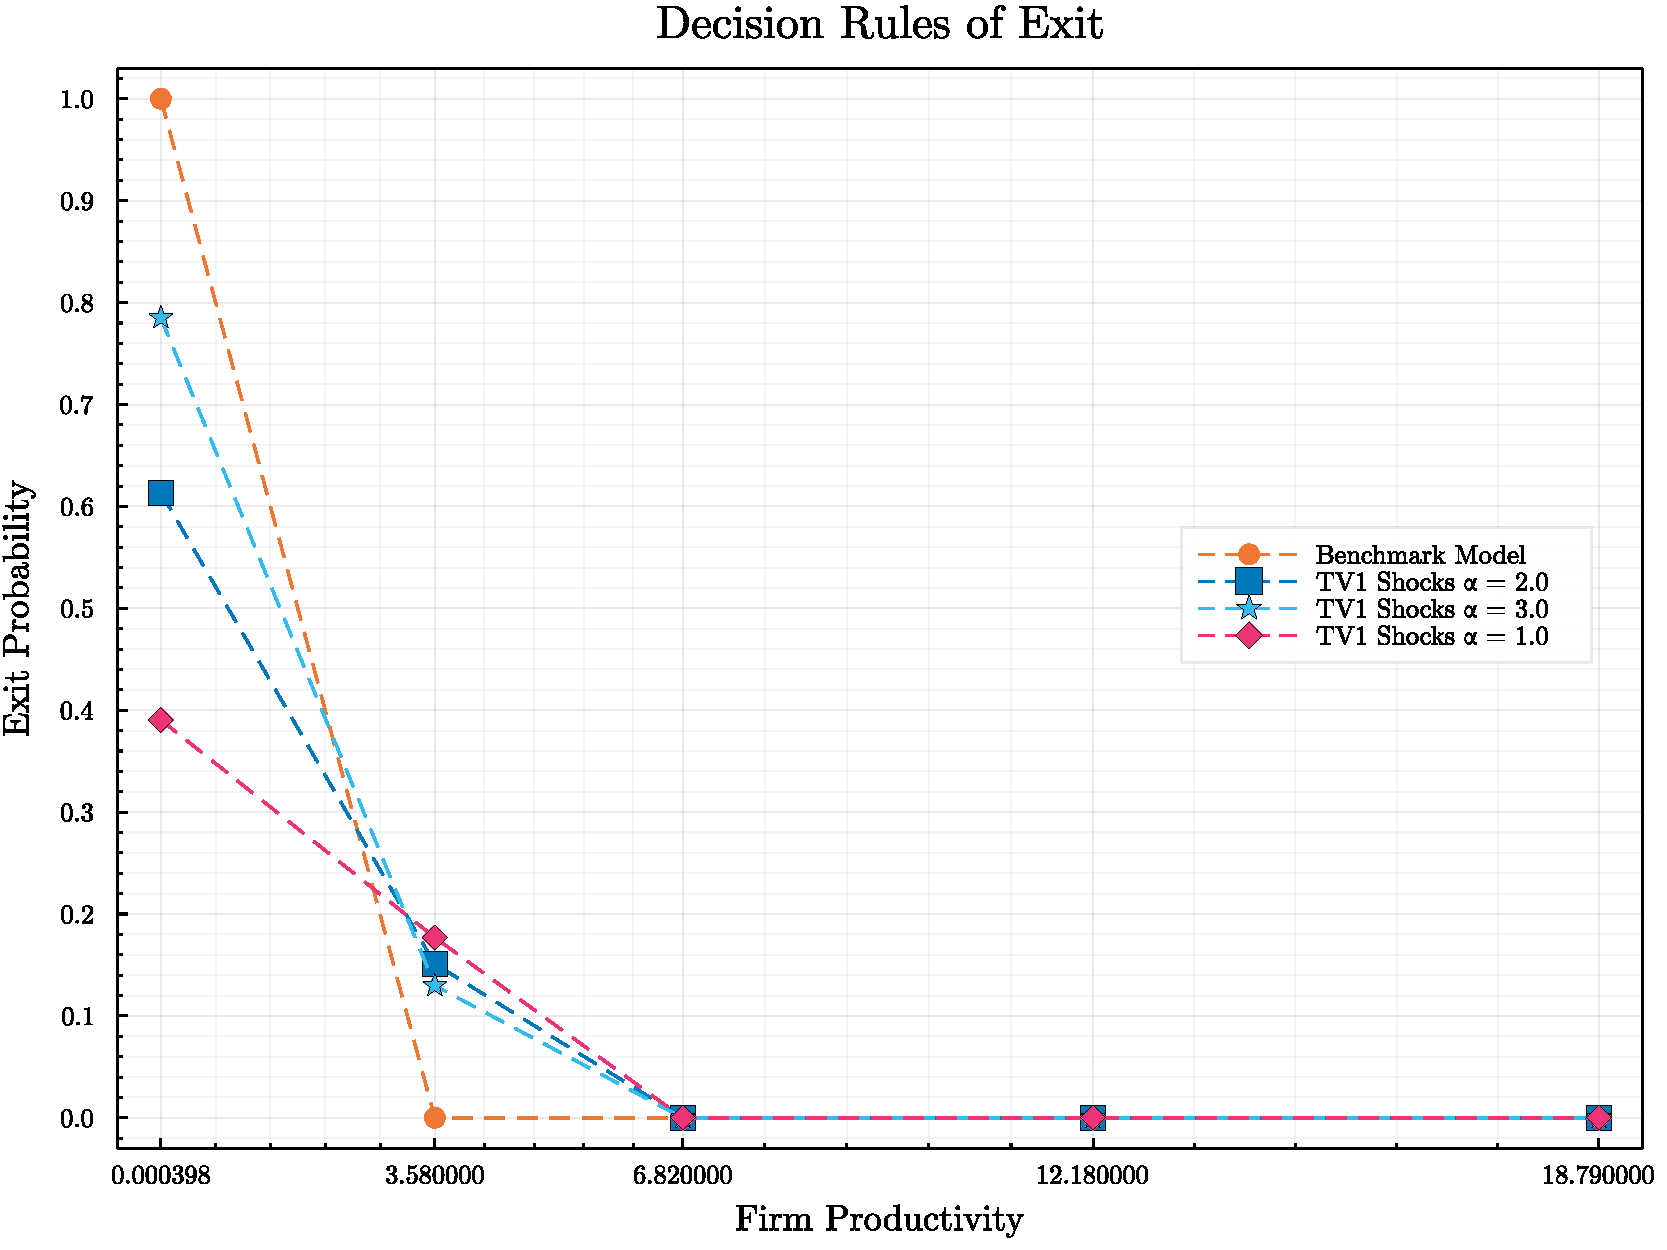
\includegraphics[scale=.35]{Figures/decision_rules.pdf}
	\caption{Decision Rules across Model Specifications}
	\label{T3}
	\end{center}
	\end{figure}
\end{solution}

\subsubsection*{Task 4}
How does the exit decision rule change if cf rises from 10 to 15?

\begin{solution}

\end{solution}

\newpage
	\section*{Appendix}
 	The first code file runs the code.
 	\jlinputlisting{Code/run_model.jl}
	
 	The second code file contains the relevant functions.
 	\jlinputlisting{Code/hopenhayn_rogerson.jl}

\end{document}